\documentclass{article}
\usepackage{graphicx}
\setlength{\textheight}{9in}
\setlength{\topmargin}{-.5in}
\setlength{\headheight}{0.25in}
\setlength{\headsep}{0.25in}
\setlength{\topskip}{0in}

% arara: pdflatex
\begin{document}

{\LARGE Automated Blocking Posterior Density Plots}

\section{Random Effects model}
\begin{figure}[h]
\centerline{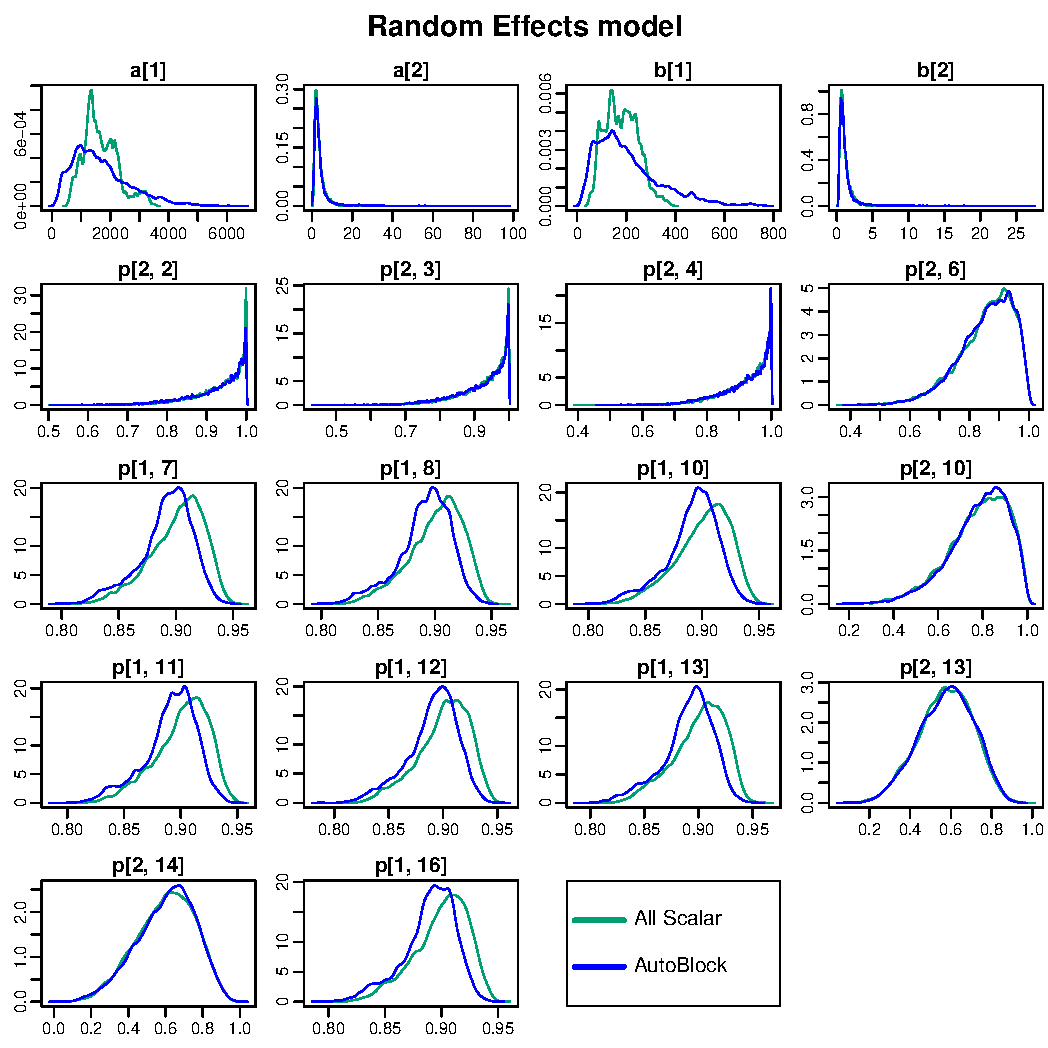
\includegraphics[scale=1.0]{RandomEffectsmodel}}
\end{figure}
\thispagestyle{empty}
\clearpage

\section{Auto-Regressive model}
\begin{figure}[h]
\centerline{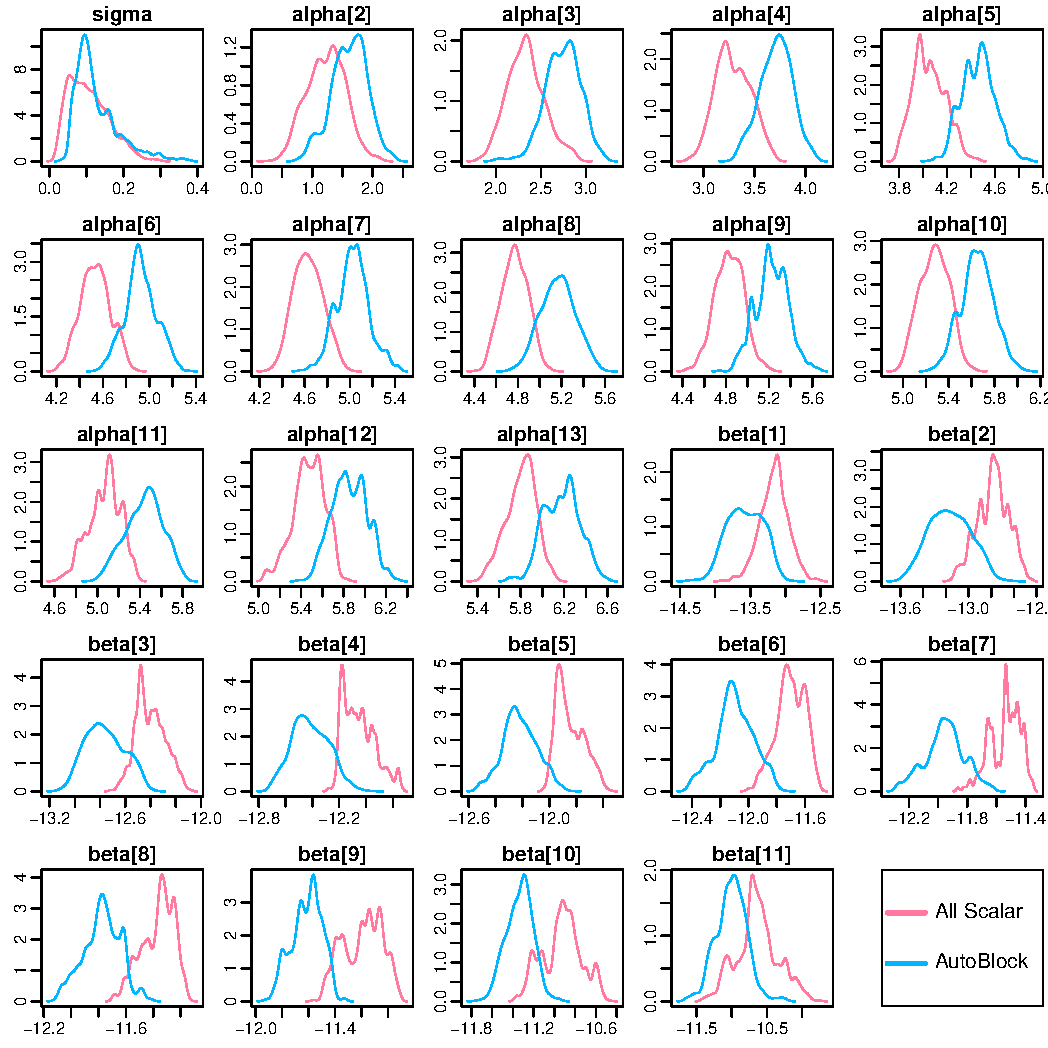
\includegraphics[scale=1.0]{AutoRegressivemodel}}
\end{figure}
\thispagestyle{empty}
\clearpage

\section{State Space model (independent)}
\begin{figure}[h]
\centerline{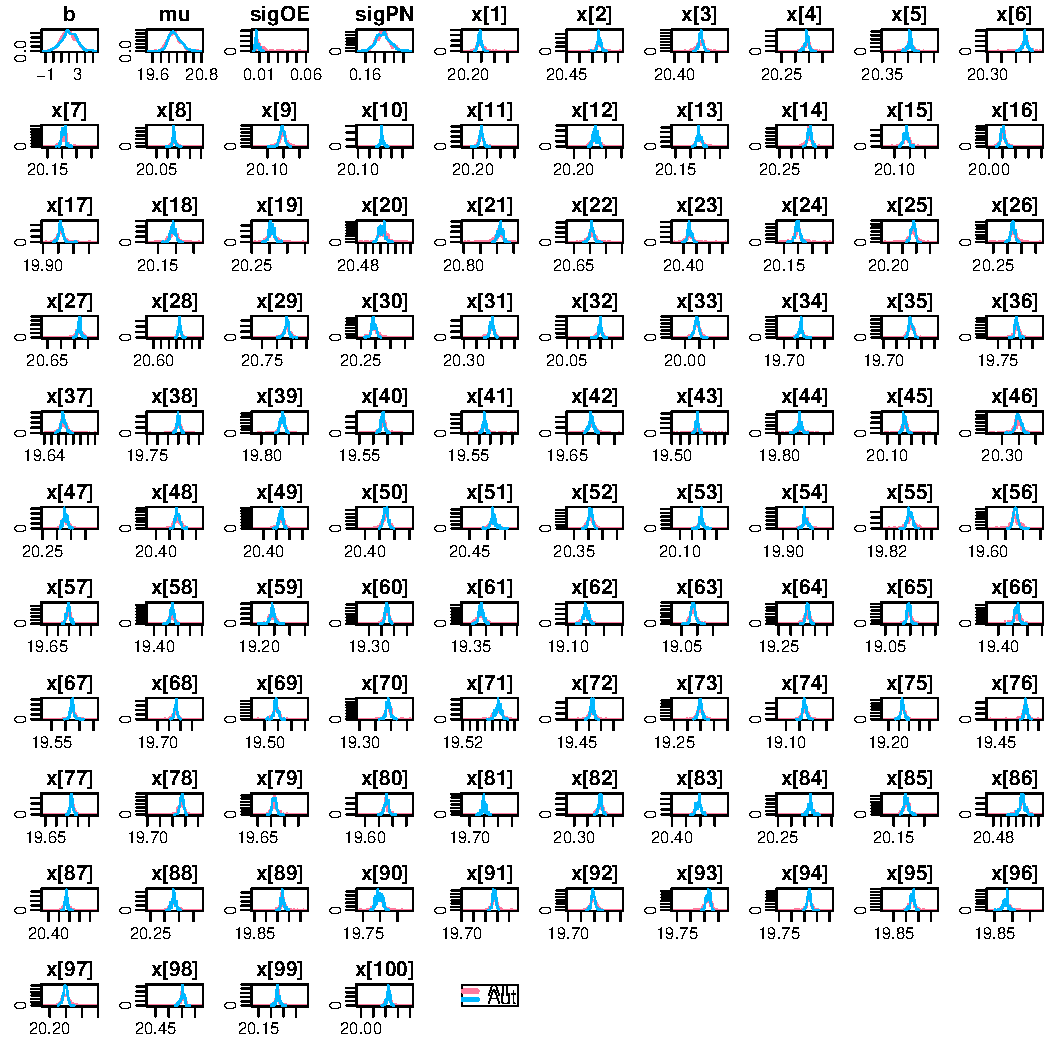
\includegraphics[scale=1.0]{StateSpacemodelindependent}}
\end{figure}
\thispagestyle{empty}
\clearpage

\section{State Space model (correlated)}
\begin{figure}[h]
\centerline{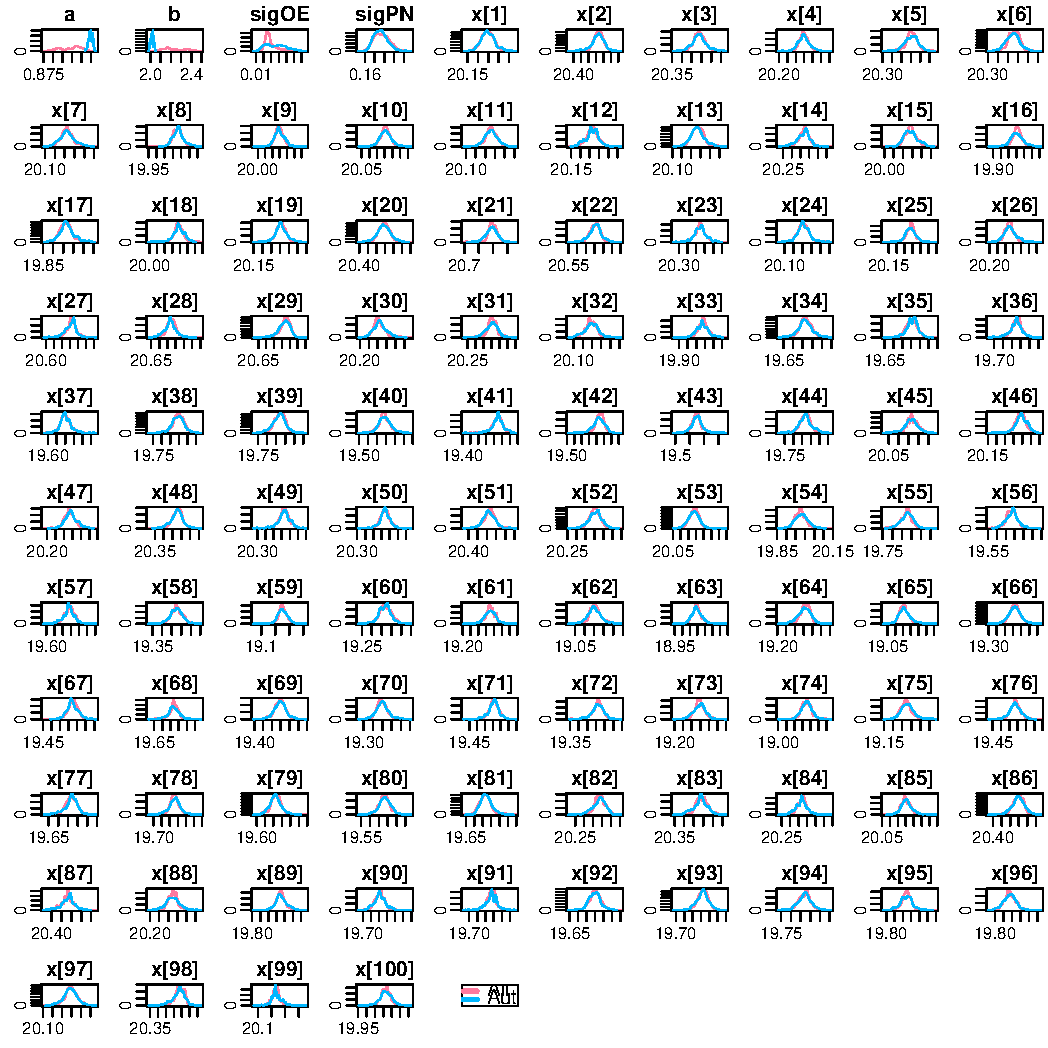
\includegraphics[scale=1.0]{StateSpacemodelcorrelated}}
\end{figure}
\thispagestyle{empty}
\clearpage

\section{Spatial model}
\begin{figure}[h]
\centerline{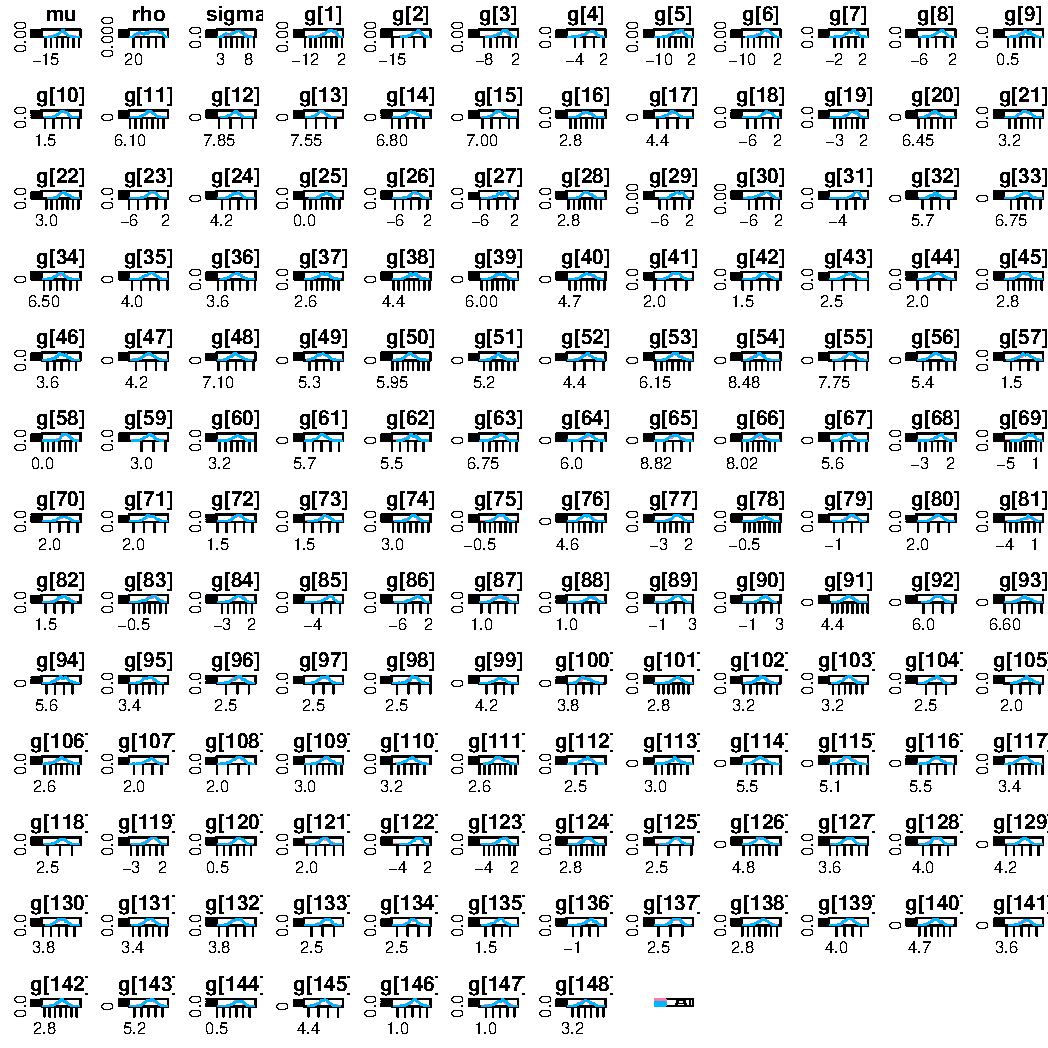
\includegraphics[scale=1.0]{Spatialmodel}}
\end{figure}
\thispagestyle{empty}
\clearpage

\section{GLMM}
\begin{figure}[h]
\centerline{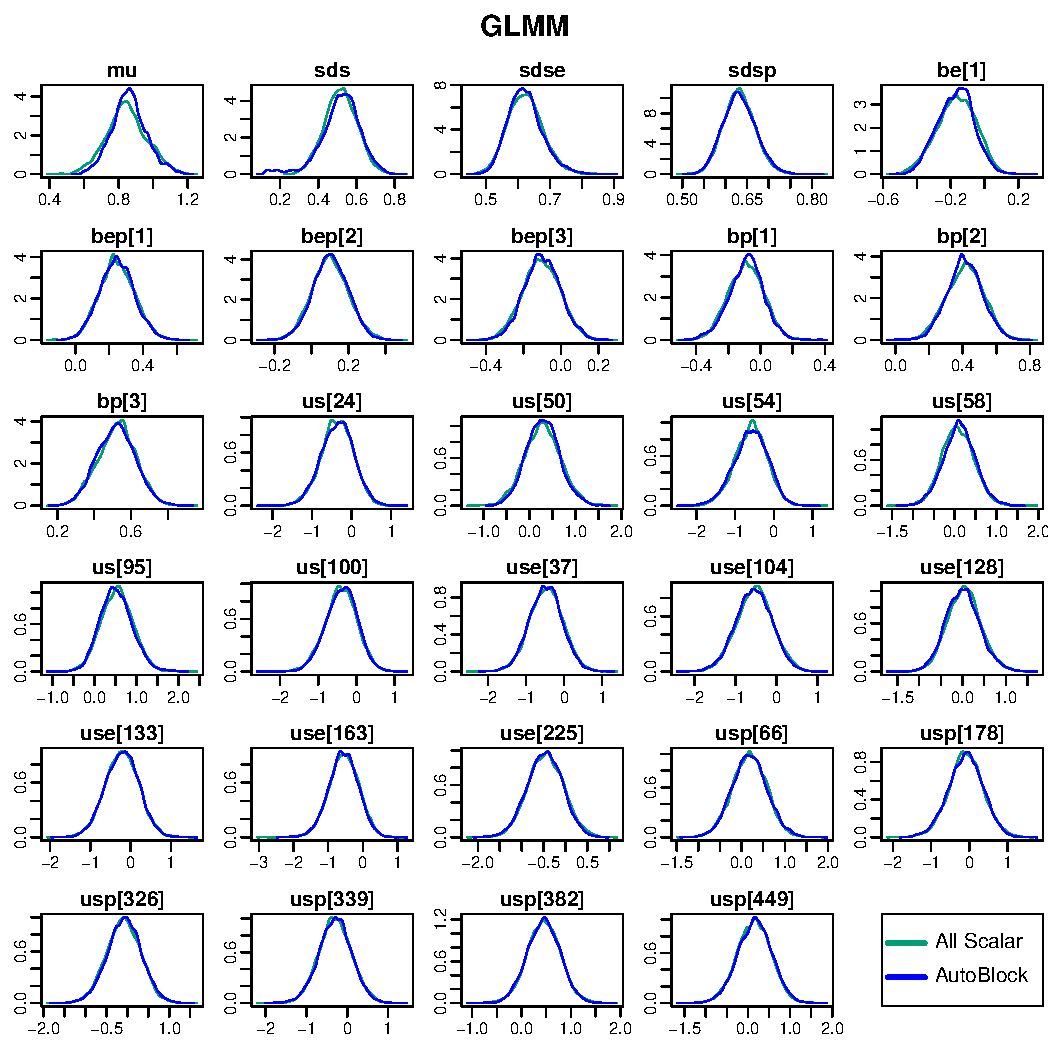
\includegraphics[scale=1.0]{GLMM}}
\end{figure}
\thispagestyle{empty}
\clearpage

\end{document}